\documentclass[pre, superscriptaddress, twocolumn,pre]{revtex4-1}
\usepackage{amsmath, amssymb, color, graphicx}
\definecolor{linkcolor}{rgb}{0,0,0.6} 
\usepackage[pdftex,colorlinks=true,
	pdfstartview = FitV,
	linkcolor    = linkcolor,
	citecolor    = linkcolor,
	urlcolor     = linkcolor,	
	hyperindex   = true,
	hyperfigures = false]{hyperref}

\newcommand{\dd}{\text{d}}
\newcommand{\ee}{\text{e}}
\newcommand{\ii}{\text{i}}


% ===============================================================================


\begin{document}

\title{How can energy flows constrain fluctuations beyond equilibrium?\\Renormalization of transport and structure in a driven liquid}

\author{Laura Tociu}
\affiliation{James Franck Institute, University of Chicago, Chicago, IL 60637}
\affiliation{Department of Chemistry, University of Chicago, Chicago, IL 60637}

\author{\'Etienne Fodor}
\affiliation{DAMTP, Centre for Mathematical Sciences, University of Cambridge, Wilberforce Road, Cambridge CB3 0WA, UK}

\author{Takahiro Nemoto}
\affiliation{Philippe Meyer Institute for Theoretical Physics, Physics Department, \'Ecole Normale Sup\'erieure \& PSL Research University, 24, rue Lhomond, 75231 Paris Cedex 05, France}

\author{Suriyanarayanan Vaikuntanathan}
\affiliation{James Franck Institute, University of Chicago, Chicago, IL 60637}
\affiliation{Department of Chemistry, University of Chicago, Chicago, IL 60637}

\begin{abstract}

In this paper we study the implications of energy flow or work done by external drives on the transport and structural properties of a liquid. First, using a theoretical model of a driven liquid, we put forward a relation between the spontaneous fluctuations, quantified by the diffusion coefficient, and the amount of work produced by an external drive, related to energy dissipation. Next, we demonstrate how the hierarchy between density correlations, which enforces the fluid structure, is now affected by sustained energy dissipation. Finally, by harvesting trajectories that preferentially dissipate or absorb energy, we predict how energy flows can renormalize the interactions between particles of the liquid. These predictions are confirmed with atomistic simulations. Together, our results show how the various emergent collective excitations in many body interacting systems can be accurately controlled or tuned at the cost of energy dissipation. 

\end{abstract}

\maketitle 


% ===============================================================================


\section{Introduction}

Non-equilibrium forces can drive novel and specific pathways to modulate self-assembly and organization in materials. The close connection between energy dissipation and organization is especially apparent in living systems~\cite{Toyabe2010, Ahmed2016, Battle604}. As an example, the flagella motors of {\it E. Coli} use non-equilibrium forces to exhibit unique phenomenology combining ultra-sensitive response, adaptation, and motor restructuring as a function of the applied torque~\cite{Lele2013, Lan2012, Wang2017}. Moreover, both {\it in vivo} studies of the cellular cytoskeleton, as well as {\it in vitro} experiments on model systems of actin and/or microtubule networks driven by molecular motors, have also shown that non-equilibrium forces control a large variety of functionality in the cell~\cite{Silva2011, Sanchez2012, Blanchoin2014, Murrell2015}. They have demonstrated, for instance, how living systems can robustly sense forces, and therefore constantly adapt to their surroundings~\cite{Decamp2015}. 


To elucidate the role of non-equilibrium forces in material properties, it is crucial to first examine how sustained energy flows affect the dynamics. While the features of equilibrium systems are well established, progress in controlling non-equilibrium systems has been hampered by a lack of general principles~\cite{Takatori2015, Cates2015, Solon2015a, Nguyen2016, Fodor2016, Murugan2017, Nguyen2018}. For instance, the canonical relation between fluctuation and dissipation no longer holds \textendash its violation is directly related to the work applied by non-equilibrium forces~\cite{Harada2005, Harada2006}. Understanding the interplay between the energy dissipated by these non-equilibrium forces and resulting structure and organization is an open and important problem~\cite{Mizuno2007, Wilhelm2008, Visco2015, Turlier2016, Nardini2017}.

Minimal models of active or driven matter can provide analytically and computationally tractable test beds to study such interplays in non-equilibrium systems~\cite{Cates2015,Han2016}. Activity or non-equilibrium drive has been shown to induce phase transitions, generate large mesoscopic currents along interfaces, and support long spatio-temporal correlations that would be extremely unlikely in sub critical classical systems with short ranged potentials~\cite{Cates2015,Han2016,Nguyen2014b}.  Recent theoretical and computational work has studied nucleation phenomena~\cite{Redner2016} and obtained expressions for pressure and other mechanical properties of active media~\cite{Solon2015a}. In spite of these advances, a microscopic theory for the tradeoffs between energy consumption and organization in active or driven media remains elusive. In this paper, we focus on developing such a microscopic theory for driven liquids, i.e. liquids in which particle are driven out of equilibrium by the action of external time dependent fields. 


%Paragraph on large deviations: cloning algorithm~\cite{Giadina2006, tailleur2007probing, Hurtado2009, Nemoto2016, Ray2018, Klymko2018, Brewer2018}, dynamical heterogeneities in glassy systems~\cite{garrahan2007, Hedges2009, Pitard2011, Speck2012, Bodineau2012a, Limmer2014, Nemoto2017}, high-dimensional chaotic chains~\cite{tailleur2007probing, laffargue2013}, clustering of active self-propelled particles 


In a recent work, some of the present authors have reported empirical connections between dissipation, structure, transport and emerging phases in a model driven system~\cite{Han2016, delJunco2018}. The empirical connections were explained using phenomenological models that did not treat the underlying dynamics explicitly. It remains to be seen if similar connections can be obtained within settings where coarse-graining and interactions between particles is treated more rigorously~\cite{Dean1996, Demery2011, Demery2014}. The connection between dissipation and structure has also been observed in other contexts. Recent work has shown that changing dissipation, by biasing trajectories externally~\cite{Lecomte2007, Touchette2009, Jack2010}, strongly affects the density correlations of non-equilibrium fluids~\cite{Nemoto2018a}. This collection of results suggest that controlling the dissipation rate can be potentially be a fruitful way to constrain the properties of emerging structures in non-equilibrium systems.


Motivated by these connections between dissipation, transport and structure, in this paper, we explore how energy flows modify the properties of a class of driven liquids. The fist system we consider is composed of a driven \textit{tracer} particle interacting with a Gaussian fluctuating field~\cite{Chandler1993, Dean1996, Demery2014, Kruger2017}. The fluctuations of the Gaussian field are meant to mimic the density fluctuations of a liquid~\cite{Chandler1993}. Our theoretical system is meant to model setups such as those introduced in Ref.~\cite{Han2016,delJunco2018} where a liquid is driven out of equilibrium through the action of a time dependent external field on select particles.  We derive expressions for the diffusion coefficient of driven \textit{tracer} particle and the work performed by the drive, in the limits of large and small drive period, by treating interactions between the tracer and Gaussian field perturbatively. In both regimes, work and diffusion exhibit the same scaling in terms of drive amplitude and period, illustrating the interplay between dissipation and transport in this non-equilibrium system. 



Next, we obtain a generic relation between work and force fluctuations, from which we explore how density correlations in the driven liquid are modified due to the non-equilibrium driving. While these relations show how energy consumption modifies the transport and structural properties of the system \textendash such relations have been used to construct composition dependent diffusion constants and explain phase transition behavior in driven systems~\cite{delJunco2018} \textendash they are perturbative in interactions and have been derived for particular non-equilibrium driving protocols. Further, they do not provide concrete intuition for how particular structures or configurations can be preferentially stabilized or self-assembled at the cost of energy consumption. 

In the last section of the paper, we attempt to address these issues and generalize the above mentioned connections by simply focussing our attention on trajectories which preferentially pump energy into or extract energy from, particular interactions in the system. On average, the trajectories sampled in the course of an equilibrium simulation conserve energy. However, by sampling rare events, trajectories that preferentially absorb or emit energy can be harvested. Such trajectories can serve as a proxy for non-equilibrium simulations in which energy is pumped into particular modes by the action of external non-conservative forces. Similar techniques have been used to mimic non-equilibrium events in glassy systems~\cite{garrahan2007,Hedges2009}. 

We use techniques from large deviation theories~\cite{garrahan2007, Hedges2009, Pitard2011, Speck2012, Bodineau2012a, Limmer2014, Nemoto2017} to generate these rare ensembles where trajectories are biased according to particular energy flow rates. Using the techniques developed in  Ref ~\cite{Chetrite2013, Jack2010}, we analytically predict the steady state configurations generated by such dynamics at weak biasing. In particular, our analytical results identify a set of renormalized inter-particle interaction potentials that can generate configurations statistically equivalent to the configurations generated by tuning energy flows. 
Direct sampling of biased trajectories using the cloning algorithm \cite{Giadina2006,tailleur2007probing,Hurtado2009,Nemoto2016,Ray2018,Klymko2018,Brewer2018} confirm that tuning energy fluxes leads to changing the fluid structure in a controlled manner as predicted by our analytical results. While our analytical results are formally valid only at weak biasing, the numerical simulations indicate that our predictions can be used to obtain qualitative intuition even at high biasing. This result shows how energy consumption can potentially be used to tailor specific interactions between particles. Having such control can potentially enable complex self-assembly at the cost of energy dissipation. 

Together, our results show how energy dissipation can modify the structure, transport properties of a fluid. They can also provide design principles for the construction of complex addressable energy landscapes at the cost of energy consumption. 


% ===============================================================================

\section{Renormalization of structure and transport properties due to energy flows}


\subsection{Renormalization of transport due to energy flows}
\subsubsection{Perturbation theory for driven tracers interacting with Gaussian fields}\label{sec:method}
In order to explore the interplay between energy consumption and diffusion, we formulate a minimal model in which a tracer particle is interacting with a liquid bath. Following equilibrium theories of density fluctuations~\cite{Chandler1993} and field theories obtained from formal coarse-graining procedures~\cite{Dean1996,Kruger2017}, we model the liquid as a Gaussian field.

To this end, we consider the following general Hamiltonian of a Gaussian density field interacting with a tracer with position ${\bf r}_0$:
\begin{equation}
	\begin{aligned}
		H &= \frac{T}{2} \int \delta \rho ({\bf r}) \chi^{-1}({\bf r} - {\bf r}') \delta \rho ({\bf r}') \dd{\bf r}\dd{\bf r}'
		\\
		&\quad + \int V({\bf r}-{\bf r}_0) \delta \rho({\bf r}) \dd{\bf r} ,
	\end{aligned}
\end{equation}
where $T$ is the bath temperature, and we have set the Boltzmann constant to unity $k_{\rm B}=1$. The density fluctuations around the average density $\rho_0$ are defined as $\delta \rho({\bf r},t ) = \rho({\bf r}, t) - \rho_0 $. The density covariance $\chi$ is written in terms of the two point correlation function $g$ as $\chi({\bf r}-{\bf r}')= \langle \delta \rho({\bf r}) \delta \rho ({\bf r}') \rangle=  \rho_0 \delta({\bf r} - {\bf r}') +\rho_0^2 g({\bf r}-{\bf r}')$.


The conserved dynamics of the density field $\delta\rho$ is given by
\begin{equation}\label{eq:EvolutionField}
	\begin{aligned}
		\frac{\partial \delta \rho({\bf r}, t)}{\partial t} &= D_{\rm G} \nabla^2 \int \chi^{-1} ({\bf r}-{\bf r}') \delta \rho({\bf r}', t) \dd{\bf r}'
		\\
		&\quad + \frac{1}{\gamma_{\rm G}} \nabla^2 V({\bf r}-{\bf r}_0(t)) + \nabla \cdot {\boldsymbol\Lambda}({\bf r},t) ,
	\end{aligned}
\end{equation}
where $D_{\rm G} = T/\gamma_{\rm G}$, and $\gamma_{\rm G}$ is the field damping coefficient. The term $\boldsymbol\Lambda$ is a zero-mean Gaussian white noise with correlations
\begin{equation}
	\langle \Lambda_\alpha({\bf r}, t) \Lambda_\beta({\bf r}', t') \rangle = 2 D_{\rm G} \delta_{\alpha\beta}\delta({\bf r} - {\bf r}')\delta(t-t') .
\end{equation}
In Fourier space, Eq.~\eqref{eq:EvolutionField} becomes
\begin{equation}\label{eq:FourierEvolutionField}
	\begin{aligned}
		\frac{\partial \delta \rho({\bf q},t)}{\partial t} &= - |{\bf q}|^2 \left[ D_{\rm G} \chi^{-1}({\bf q}) \delta \rho({\bf q},t) + \frac{V({\bf q})}{\gamma_{\rm G}} \ee^{-\ii {\bf q} \cdot {\bf r}_0(t)} \right]
		\\
		&\quad + \ii{\bf q}\cdot{\boldsymbol\Lambda} ({\bf q},t) ,
	\end{aligned}
\end{equation}
where $\delta\rho({\bf q},t)=\int\rho({\bf r},t){\rm e}^{-{\rm i}{\bf q}\cdot{\bf r}} {\rm d}{\bf r}$.


The complementary equation of motion for the tracer reads
\begin{equation}\label{eq:EvolutionTracer}
	\dot{\bf r}_0 = \frac{1}{\gamma} \left( {\bf F}_\text{c}+{\bf F}_\text{d} \right) + {\boldsymbol\eta_0} ,
\end{equation}
where $\gamma$ is the tracer friction coefficient. The conservative force ${\bf F}_\text{c}$ embodies the interaction with the field $\delta\rho$:
\begin{equation}
	{\bf F}_\text{c}(t) = - \int \ii{\bf q} V(-{\bf q})\ee^{\ii{\bf q} \cdot {\bf r}_0(t)} \delta \rho({\bf q}, t) \frac{\dd{\bf q}}{(2\pi)^d} ,
\end{equation}
where $d$ refers to the spatial dimension. The term ${\boldsymbol\eta}_0$ is a zero-mean white Gaussian noise with correlations
\begin{equation}
	\langle\eta_{0\alpha}(t)\eta_{0\beta}(0)\rangle = 2 D_0 \delta_{\alpha\beta}\delta(t) ,
\end{equation}
where $D_0 = T/\gamma$.


The tracer is driven out of equilibrium by the driving force ${\bf F}_\text{d}$, taken in two dimensions as
\begin{equation}\label{eq:theta}
	{\bf F}_{\rm d}(t) = f \big[\sin(\omega t) \hat{\bf e}_x + \cos(\omega t)\hat{\bf e}_y \big] ,
\end{equation}
where $f$ and $\omega$ are respectively the amplitude and the frequency of the drive. The drive persistence time $\tau$ is then defined as $\tau=2\pi/\omega$. The relative strength of the drive can be expressed in terms of the P\'eclet number $\text{Pe}$, defined as $\text{Pe} = \sigma f/\gamma D_0$, where $\sigma$ is the typical tracer size~\cite{Han2016, delJunco2018}. In the absence of interactions with the field $\delta\rho$, the average tracer position follows a periodic orbit, corresponding to a circle in two dimensions.


The field dynamics~\eqref{eq:FourierEvolutionField} can be exactly solved. Specifically, by labeling $\chi^{-1}({\bf q}) = K({\bf q})$, we get
\begin{equation}
	\begin{aligned}
		\delta\rho({\bf q},t) &= \int_{-\infty}^t \dd s \ee^{-D_{\rm G} |{\bf q}|^2 K({\bf q})(t-s)}
		\\
		&\quad\times \left[ \ii{\bf q} \cdot {\boldsymbol\Lambda}({\bf q},s) - |{\bf q}|^2 \frac{V({\bf q})}{\gamma_{\rm G}} \ee^{-\ii {\bf q}\cdot {\bf r}_0(s)}\right] ,
	\end{aligned}
\end{equation}
yielding
\begin{equation}\label{eq:ConservativeForce}
	\begin{aligned}
		{\bf F}_\text{c}(t) &= \int \frac{\dd{\bf q}}{(2\pi)^d} \ii{\bf q} V(-{\bf q}) \ee^{\ii{\bf q} \cdot {\bf r}_0(t)} \int_{-\infty}^t \dd s \ee^{-D_{\rm G} |{\bf q}|^2 K({\bf q})(t-s)}
		\\
		&\quad\times \left[ |{\bf q}|^2 \frac{ V({\bf q})}{\gamma_{\rm G}} \ee^{-\ii{\bf q} \cdot {\bf r}_0(s)} - \ii{\bf q} \cdot {\bf\Lambda}({\bf q}, s) \right] .
	\end{aligned}
\end{equation}
Then, the tracer dynamics given by~\eqref{eq:EvolutionTracer} and~\eqref{eq:ConservativeForce} is written in a closed form, namely independently of the density field $\delta\rho$.


Following stochastic thermodynamics~\cite{Sekimoto1998, Seifert2012}, the average rate at which energy is dissipated into the thermostat $\cal J$ is simply defined as the power of the forces exerted by the driven tracer on the solvent: ${\cal J} = \gamma \langle\dot{\bf r}_0\cdot(\dot{\bf r}_0-{\boldsymbol\eta}_0)\rangle$. It can be separated into free motion and interaction contributions as ${\cal J} = f^2/\gamma - \dot w$, where
\begin{equation}\label{eq:work}
	\dot{w} = -\frac{1}{\gamma} \langle{\bf F}_\text{c}\cdot {\bf F}_\text{d}\rangle .
\end{equation}
Then, the rate of work $\dot w$ is the main quantity of interest to investigate how dissipation relates with properties of the system.


In this work, we have simply proposed the dynamics in~\eqref{eq:EvolutionField} starting from a Gaussian field theory for density fluctuations.  Using a systematic coarse-graining procedure~\cite{Dean1996}, the dynamics for the density field of the undriven particles can in fact be derived in terms of pair-wise potential $V$. The linearization around the average value $\rho_0$ leads to~\eqref{eq:FourierEvolutionField}, where $D_{\rm G}=\rho_0D_0$, $\gamma_{\rm G}=\gamma/\rho_0$ and $\chi^{-1}({\bf q}) = 1/\rho_0 + V({\bf q})/D_0$~\cite{Demery2011, Demery2014}. In practice, such a density dynamics should only be valid for weak interactions {\it a priori}, yet previous works have shown that it remains qualitatively relevant even beyond this regime~\cite{Demery2015, Martin2018, Nemoto2018a}. Indeed, Gaussian field theories for density fluctuations provide a very good description of the thermodynamics of liquids~\cite{Chandler1993}.


% -------------------------------------------------------------------------------




%\begin{figure}
%	\centering
%	\includegraphics[width=.95\linewidth]{D_active_vs_Pe_10p4.pdf}
%	\includegraphics[width=.95\linewidth]{dwvsPe.pdf}
%	\caption{\label{fig:diffusion}
%		(Top) Diffusion coefficient $D$ of driven particles as a function of $\rm Pe$, for $\tau= 20$ (green), $30$ (yellow) and $40$ (blue). Here, $\text{Pe}$ is the P\'eclet number and is defined as $\text{Pe} = \sigma A/\gamma D_0$, where $\sigma$ is the typical tracer size. The lines are fits to the functional form $D = D_{\rm eq} + a(\tau) {\rm Pe} + b(\tau) {\rm Pe}^2$ with $a(20)/b(20)\approx -0.04$, $a(30)/b(30)\approx -0.09$, $a(40)/b(40)\approx 0.25$. (Bottom) $\langle \dot{w} \rangle$ as a function of $Pe$ for the same range of values of $\tau$. The lines are fits of $\langle \dot{w} \rangle$ to quadratic functions of $Pe$, $\langle \dot{w}\rangle \propto Pe^2$. 
%	}
%\end{figure}


% ===============================================================================

\subsubsection{Energy flows control spontaneous diffusion}\label{sec:diff}

Our first aim is to derive explicit expressions for the tracer diffusion coefficient $D$, defined as $D = \underset{t\to\infty}{\lim} (1/2dt) \big\langle \big[\langle{\bf r}_0(t)\rangle-{\bf r}_0(t)\big]^2 \big\rangle$, and the rate of dissipated work $\dot w$ given in~\eqref{eq:work}. The tracer dynamics, given in its closed form by~\eqref{eq:EvolutionTracer} and~\eqref{eq:ConservativeForce}, can be used to set up a perturbation in terms of the interactions between the tracer and the density field $\delta\rho$. Following~\cite{Demery2011, Demery2014}, we then scale the potential $V$ by a small parameter $h$ in~\eqref{eq:ConservativeForce}, so that the tracer is uncoupled from the bath when $h=0$. We also present all our results in terms of $K({\bf q}) = \chi^{-1}({\bf q})$, where $\chi({\bf q})$ is the Fourier transform of the two point density-density correlation function $\chi({\bf r}-{\bf r}')= \langle \delta \rho({\bf r}) \delta \rho ({\bf r}')\rangle$, as defined in Sec.~\ref{sec:method}. 


The perturbation theory detailed in Appendix~\ref{app:diff} allows us to extract how the rate of work $\dot w$ performed on the system and the diffusion coefficient $D$ scale in various limits. We first consider the limit of high frequencies $\omega\tau_{\rm R}\gg 1$, where the relaxation time scale $\tau_{\rm R}=(D_{\rm G}/\sigma^2)K(|{\bf q}|=1/\sigma)$ controls the diffusion of the density field over the tracer size $\sigma$, and of small P\'eclet number ${\rm Pe}\ll 1$. In this regime, the rate of work applied on the driven tracer scales like
\begin{equation}\label{eq:w_small}
	\dot w = \frac{(D_0 hPe)^2}{d\omega^2\gamma\sigma^2} \int|{\bf q}|^4 |V({\bf q})|^2 \frac{D_0 + D_{\rm G}K({\bf q})}{D_0K({\bf q})} \frac{\dd{\bf q}}{(2\pi)^d} .
\end{equation}
Besides, the increase of the diffusion coefficient $D-D_{\rm eq}$ scales like 
\begin{equation}\label{eq:D_small}
	D-D_{\rm eq} = \frac{(D_0 h Pe)^2}{d\omega^2\gamma^2\sigma^2} \int\frac{|{\bf q}|^2 |V({\bf q})|^2 } {K({\bf q})\big[D_0 + D_{\rm G} K({\bf q})\big]} \frac{\dd{\bf q}}{(2\pi)^d} ,
\end{equation}
where $D_{\rm eq}$ is the diffusion constant of the tracer particle under equilibrium conditions, namely when $f=0$. These results are valid to quadratic order in $\rm Pe$ and in $h$, the parameter that sets the strength of coupling between the tracer and the bath.


When the size $a$ of the bath particles is significantly smaller than the tracer size $\sigma\gg a$, one can safely neglect the variation of $K({\bf q})$ in~(\ref{eq:w_small}-\ref{eq:D_small}), such as $K({\bf q}) \simeq K(|{\bf q}|=1/a)$. Then, the renormalization of the diffusion coefficient $D-D_{\rm eq}$ can be simply written in terms of the rate of work $\dot w$: 
\begin{equation}\label{eq:work_D}
	\frac{D-D_{\rm eq}}{\sigma^2} \sim \frac{1}{\big[1+\rho_0K(|{\bf q}|=1/a)\big]^2} \cdot \frac{\dot w}{T} ,
\end{equation}
where we have used $D_{\rm G}=\rho_0 D_0=\rho_0 T/\gamma$. Thus, the excess rate at which the tracer moves over its own size compared to equilibrium, set by the lhs of~\eqref{eq:work_D}, is controlled by the rate at which work is applied on the tracer, set by the rhs of~\eqref{eq:work_D}. The proportionality factor is determined by the details of the bath-tracer interactions $V$ and of the density fluctuations $K$.


In the opposite limit, namely at low frequencies $\omega\tau_{\rm R}\ll 1$ and small P\'eclet number ${\rm Pe}\ll1$, we get
\begin{equation}\label{eq:w_large}
	\dot w = \frac{(D_0 hPe)^2}{d\gamma\sigma^2} \int \frac{|V({\bf q})|^2}{D_0K({\bf q}) \big[D_0 + D_{\rm G}K({\bf q})\big]} \frac{\dd{\bf q}}{(2\pi)^d} .
\end{equation}
The rate of work $\dot w$ is now independent of the driving frequency $\omega$.  Similarly, we obtain the renormalization of diffusion coefficient $D-D_{\rm eq}$ as
\begin{equation}\label{eq:D_large}
	D - D_{\rm eq} = \frac{5(D_0 hf)^2}{d\gamma^2\sigma^2} \int \frac{|V({\bf q})|^2/|{\bf q}|^2}{K({\bf q})\big[D_0 + D_{\rm G}K({\bf q})\big]^3} \frac{\dd{\bf q}}{(2\pi)^d} .
\end{equation}
Again, Eq.~\ref{eq:w_large} and Eq.~\ref{eq:D_large} are valid to order $h^2$ and ${\rm Pe}^2$.To this order in $h$, the scaled work $\gamma\dot w/f^2$ coincides with the reduced equilibrium diffusion $D_{\rm eq}/D_0-1$~\cite{Demery2011, Demery2014}, as expected from linear response.
Our perturbation theory hence shows that scalings of $\dot w$ and $D-D_{\rm eq}$ are identical, both in terms of the drive amplitude $f$ and of its frequency $\omega$. In the regime of scale separation between tracer and bath particles $\sigma\gg a$, we can further connect work and diffusion in the same way as in~\eqref{eq:work_D}.
\begin{figure}[tbp]
\centering
\includegraphics[width=0.85\linewidth]{dw_fvar_10p_active_av_active.eps}
\caption{Rate of work as a function of the renormalization of force fluctuations. The averages are taken over the active particles in a simulation with 10\% active particles. The data sets correspond to tau values of 20, 30, 40 and 50, and the sampled Pe values were 6, 12, 18, 24, 30 and 36. Eq.~\ref{eq:V2} is satisfied with $\gamma=100$.}
\label{fig:dw_fvar}
\end{figure}


% ===============================================================================


\subsection{Energy flows change the\\fluid structure}

We now explore how energy flows affect the liquid structure by modifying the density correlations. To this aim, we begin by treating each of the bath particles individually (instead of using the Gaussian field theory developed in the previous section) and express the conservation of tracer-bath interaction energy, 
\begin{equation}
V=\sum_{i=1}^{N} v({\bf r}_i,{\bf r}_0)\,,
\label{eq:Vdef}
\end{equation}where $v({\bf r}_i,{\bf r}_0)$ is the interaction energy between the tracer particle at ${\bf r}_0$ and a bath particle at ${\bf r}_i$ and $N$ is the number of bath particles, using It\^o calculus:
\begin{equation}\label{eq:V1}
	\frac{\dd\langle V\rangle}{\dd t} = 0 =\sum_{i=0}^N \langle\dot{\bf r}_i\circ\nabla_iV\rangle + D_0 \langle\nabla_i^2V\rangle ,
\end{equation}
where $\circ$ denotes a product within It\^o convention, instead of the Stratonovitch convention used implicitly in the rest of the paper. Substituting the microscopic dynamics~\eqref{eq:xEOM}, using $\langle{\boldsymbol\eta_i}\circ\nabla_i V\rangle=0$, and working in the limit of low density or weak tracer bath and bath bath interactions, we get 
\begin{equation}\label{eq:V2}
	\langle \dot w\rangle = \frac{2}{\gamma} \left[ \langle{\bf F}^2 \rangle-\langle F^2\rangle_0\right] +O(h^3),
\end{equation}
where we have used the definition~\eqref{eq:work} for the rate of work $\dot w$, $\langle F^2\rangle_0 = T \langle\nabla^2_0 V\rangle$, ${\bf F}=-\nabla_0 V$ is the conservative force acting on the tagged tracer particle. We note that distinct from the usual Harada-Sasa relation~\cite{Harada2005,Harada2006}, Eq.~\ref{eq:V2} relates the work performed on a single tracer particle to the statistics of its force fluctuations. While Eq.~\ref{eq:V2} has been derived in a weak interacting limit, simulations of the driven tracer system show that it is valid in the strongly interaction limit (Fig.~\ref{fig:dw_fvar}). 

Eq.~\ref{eq:V2} can be rewritten in terms of two and three body correlation functions, 
\begin{equation}\label{eq:balance}
	\begin{aligned}
		\frac{\gamma \dot w}{2} &= \rho_0 \int \left[T \nabla^2 u({\bf r}) - (\nabla u({\bf r}))^2\right] g({\bf r}) \dd{\bf r} ,
		\\
		&\quad - \rho_0^2 \iint \left[\nabla u({\bf r})\right] \cdot \left[\nabla u({\bf r}')\right] g_3({\bf r}, {\bf r}') \dd{\bf r} \dd{\bf r}' ,
	\end{aligned}
\end{equation}
where $g$ and $g_3$ respectively refer to the two-point and the three-point density correlations. Here, $g_3$ has been defined assuming that the tracer particle is at at the origin. For a vanishing rate of work $\dot w = 0$, one recovers the first relation of the Yvon-Born-Green hierarchy between density correlations, valid for an equilibrium fluid, as expected~\cite{Hansen2013}. At finite rate of work $\dot w\neq0$, the relation between density correlations is now constrained by the amount of energy exchanged between the thermostat and the particles.


To explore the implications of the energy balance condition~\eqref{eq:balance} on the structure of the liquid, we decompose the nonequilibrium correction to the density pair correlation $g-g_{\rm eq}$ into an isotropic component $\Delta$, that depends only on $|{\bf r}|$, and an anisotropic component ${\rm Pe}.\Omega$ as
\begin{equation}\label{eq:g_dec}
	g({\bf r}) = g_{\rm eq}({\bf r}) + \Delta({\bf r}) + {\rm Pe}.\Omega({\bf r}) ,
\end{equation}
where
\begin{equation}\label{eq:Deltadef}
	\Delta({\bf r}) = \int \left[g({\bf r}) - g_{\rm eq}({\bf r}) \right] \frac{\dd\theta}{2\pi} .
\end{equation} 
We have explicitly included the $\rm Pe$ scaling in $\Omega$ motivated by the ${\rm Pe}^2$ scaling exhibited by the work.  From the definition of the isotropic component $\Delta$ in Eq.~\ref{eq:Deltadef}, it is clear that $\int\Omega({\bf r}){\dd\theta}=0$ 


\begin{figure*}
	\centering
	\includegraphics[width=\linewidth]{integral_A2.pdf}
	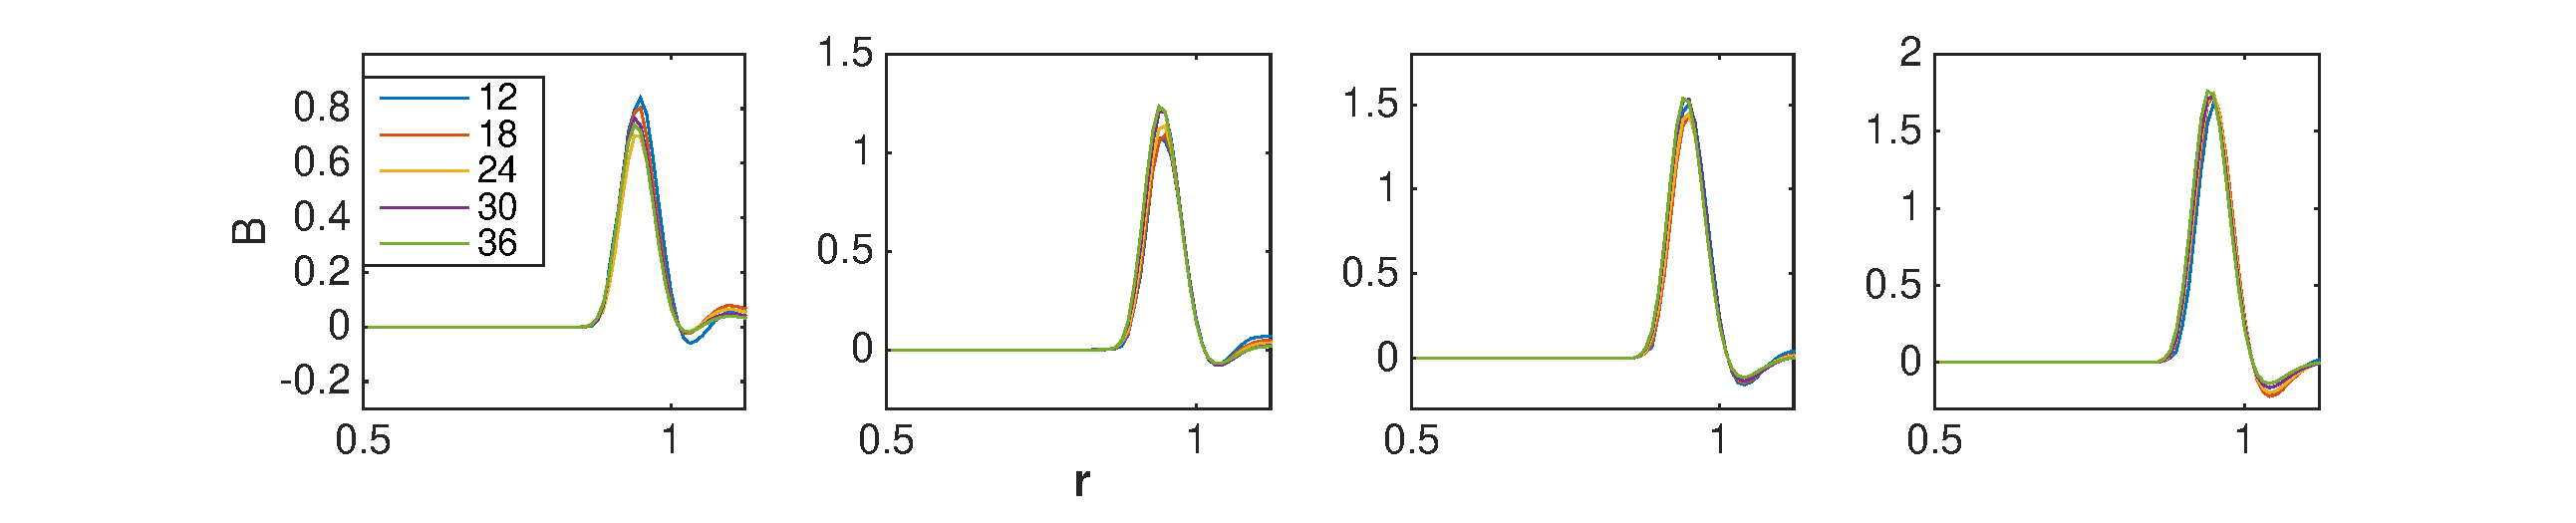
\includegraphics[width=1.0\linewidth]{del_u_sq-del_sq_u_overPesq.eps}
	\caption{\label{fig:kirk}
		(Top) Plot of ${\cal I} = \rho_0 \int \left[ T\nabla^2 u({\bf r}) - (\nabla u({\bf r}))^2\right] \Delta({\bf r}) \dd{\bf r}$ as a function of $\rm Pe$ at $\tau=\{20,30,40,50\}$, respectively from left to right. Fits are to ${\cal I} = a {\rm Pe} + b {\rm Pe}^2$. The maximum value of the ratio $b/a$ is $b/a \approx 5$ implying that the quadratic component is dominant for larger values of $Pe$. 
		(Bottom) Plot of $(1/{\rm Pe})^2 \left[T \nabla^2 u - (\nabla u)^2\right]$ as a function of the interparticle distance $r$ scaled by the particle diameter $\sigma=1$, for different values of ${\rm Pe}$. The four plots correspond to $\tau =\{20,30,40,50\}$, respectively from left to right.
	}
\end{figure*}


To proceed further, we adapt Kirkwood's closure to approximate the three-body correlation $g_3$ in terms of some two-body correlations $g$. Specifically, we assume that $g_3({\bf r},{\bf r}') = c g_{\rm eq}({\bf r} - {\bf r}') g({\bf r}) g({\bf r}')$, where $c$ is a normalization factor that satisfies $g_3({\bf r} , {\bf r}') = c g_{\rm eq}({\bf r} - {\bf r}')g_{\rm eq}({\bf r})g_{\rm eq}({\bf r}')$ at equilibrium. Using the decomposition of $g$ in~\eqref{eq:g_dec}, we only keep terms up to order $\Delta $ in the isotropic correction. We first note that the terms involving a single factor of the anisotropic contribution $\Omega$ cancel to zero upon integration from symmetry considerations. Then, the only terms that survive are either quadratic in ${\rm Pe}.\Omega({\bf r})$ or linear in $\Delta({\bf r})$:
\begin{equation}\label{eq:Kirkwood}
	\begin{aligned}
		\frac{\gamma\dot w}{2} &= \rho_0\int \left[T\nabla^2 u({\bf r}) - (\nabla u({\bf r}))^2 \right] \Delta({\bf r}) \dd{\bf r} 
		\\
		&\quad - c \rho_0^2 \iint\dd{\bf r}\dd{\bf r}' \left[\nabla u({\bf r})\right] \cdot \left[\nabla u({\bf r}')\right] g_{\rm eq}({\bf r}-{\bf r}')
		\\
		&\qquad\times \big[ 2 \Delta({\bf r}) g_{\rm eq}({\bf r}') + {\rm Pe}^2 \Omega({\bf r}) \Omega({\bf r}') + {\cal O}(\Delta^2) \big] .
	\end{aligned}
\end{equation}
This is an integral equation relation between $\Delta$, $\delta$ and $\dot w$. Starting from the condition of energy balance~\eqref{eq:balance}, it provides an explicit constraint on how the density pair correlation $g$ is modified due to non-equilibrium driving. 


In order to probe the renormalization of the structure due to the non-equilibrium driving, we compute the isotropic component $\Delta$ of the nonequilibrium correction to density pair correlations $g-g_{\rm eq}$ from direct simulations of the microscopic dynamics~\eqref{eq:xEOM}. Then, we measure ${\cal I} = \rho_0 \int \left[ T\nabla^2 u({\bf r}) - (\nabla u({\bf r}))^2\right] \Delta({\bf r}) \dd{\bf r}$ as a function of $\rm Pe$ for various values of $\tau$. The choice of the specific combination ${\cal I}$ was motivated by the fact that in the limit of low density $\rho_0 \ll 1$ and weak tracer bath interactions, $h\ll 1$ Eq.~\ref{eq:Kirkwood} implies that ${\cal I}\propto \dot{w}\propto Pe^2$ to leading order in density and interaction strength.   

We observe that $\cal{I}$ scales linearly with $\rm Pe$ in the low $\rm Pe$ region, and scales quadratically in the high $\rm Pe$ region as reported in Fig.~\ref{fig:kirk}. Given that $\dot w = {\cal O}({\rm Pe}^2)$, the linear regime is not consistent with~\eqref{eq:Kirkwood}, thus suggesting a breakdown of the underlying closure relations, such as the Kirkwood approximation. In Fig.~\ref{fig:kirk}, we show that the integrand of $\cal I$ is well approximated by a scaling as ${\rm Pe}^2$ for ${\rm Pe}>30$. In short, while such a scaling is only confirmed numerically for large $\rm Pe$, our results suggest that~\eqref{eq:Kirkwood} is indeed useful to anticipate some constraints on the renormalization of density correlations due to nonequilibrium driving.

The results of this section show how energy flows can modify the transport properties of a liquid. They also show how constraints on the structure of a non-equilibrium fluid can be obtained. These results can be used to obtain a qualitative of how non-equilibrium forces can be used to control the properties of the driven liquid. In the next section, we seek to quantify the correlations between energy consumption and structural reorganization using the framework of large deviation theories. 
% ===============================================================================


\section{Biasing with energy flows renormalizes interactions}
\label{sec:bias}
To explore how energy flows affect the microscopic interactions, we now consider biasing the dynamics in terms of the rate of change of the potential energy stored in the tracer-bath interactions, $\dd V/\dd t$. Specifically, we seek to bias the distribution of trajectories seen over the course of a simulation so that trajectories supporting energy flows are harvested preferentially.  We focus on the the tracer-bath interactions because the non conservative forces introduced in the last section act directly on these interactions. 

In order to generate such biased ensembles, we rely on the framework of large deviation theory~\cite{Chetrite2013, Jack2010}. Formally, it consists in modifying the particle trajectories by  introducing an exponential weighting function $\ee^{ k . \varepsilon(t) }$ in the path probability of the dynamics. The variable $\varepsilon$ is extensive in time, and its rate $\varepsilon(t)/t$ is controlled by the bias amplitude $k$ at large times. Therefore, biased ensembles enable one to probe a configuration associated with a specific value of $\varepsilon(t)/t$ by monitoring the external parameter $k$.



In order to bias the rate of change of the potential energy stored in the tracer-bath interactions, we chose $\varepsilon$ as
\begin{equation}\label{eq:eps}
	\varepsilon(t) = \frac{1}{\gamma} \int_0^t \left[ T\nabla_i^2 V + (\nabla_i V)\cdot({\bf F}_{{\rm d},i}+{\bf F}_i) \right] \dd s ,
\end{equation}
where ${\bf F}_i$ is the conservative force acting on particle $i$ and $i=0$ denotes the tracer particle. With this definition, $\varepsilon(t)/t \underset{t\to\infty}{\longrightarrow} \langle\dd V/\dd t\rangle_k$ according to Eqs.~(\ref{eq:V1}-\ref{eq:V2}), where $\langle\cdot\rangle_k$ denotes an average in the biased ensemble. In the unbiased case $k=0$, the energy flow vanishes $\langle\dd V/\dd t\rangle_0 = 0$. By tuning $k$ positive or negative, we generate trajectories that preferentially cause energy flow into or extract energy from the tracer-bath interactions, respectively for $\langle\dd V/\dd t\rangle_k>0$ and $\langle\dd V/\dd t\rangle_k<0$. Hence, sampling this ensemble of trajectories provides a way to assess how energy flows modify interactions specifically. We note that such trajectory biases have been used in other contexts for instance to explore dynamical heterogeneities in glassy systems~\cite{garrahan2007,Hedges2009,Pitard2011,Speck2012,Bodineau2012a,Limmer2014,Nemoto2017}, soliton solutions in high-dimensional chaotic chains~\cite{tailleur2007probing,laffargue2013} and the clustering of active self-propelled particles~\cite{Cagnetta2017,Whitelam2018,nemoto2018optimizing}.
\begin{figure*}
	\centering
	\includegraphics[width=0.99\linewidth]{Fig3Full.pdf}
	\caption{\label{fig:energybias}
		(a,b) Plot of $\langle\dot{\epsilon}\rangle$ as a function of the biasing field $k$. The driving force $Pe$ was turned off in these simulations.  Estimates of $\langle\dot{\epsilon}\rangle$ were obtained both from simulations of the biased ensemble using the cloning algorithm and from equilibrium simulations with Eq.~\ref{eq:effectivedynamics}. The two estimates are in good agreement. Together, these results show how energy biasing can modify the structure of the fluid. For values of $k>0$ when energy is pumped into the tracer bath interactions, the tracer and bath particles effectively repel each other more strongly in agreement with Eq.~\ref{eq:effectivedynamics}. Such enhanced repulsion can potentially favor phase separation of the tracer from the bath if there is a substantial concentration of tracers in the system.
		(c,d) Plot of the tracer bath pair correlation function as a function of $k$. The driving force $Pe$ was turned off in these simulations. Estimates of the pair correlation function were obtained both from simulations of the biased ensemble and from equilibrium simulations with Eq.~\ref{eq:effectivedynamics}. The two estimates are in good agreement. }
\end{figure*}

The connections demonstrated in the previous section, between diffusion of the tracer particles and work done on the system by the non-equilibrium forces, motivate our biased ensemble studies. Specifically, the connection between diffusion and work implies that the diffusion constant of the tracer is dependent on the local tracer bath compositions. Such a composition dependent diffusion constant can lead to non-equilibrium steady state configurations in which the tracer and bath particles phase separate~\cite{delJunco2018}. In effect, energy flow through the liquid seemingly generates steady state configurations resembling the steady state of an equilibrium system with enhanced tracer bath repulsions. Using the formalism of large derivation theory we now explore the implications of systematically harvesting trajectories that pump energy into or extract energy from the tracer-bond interactions. Our goal is to understand how a variety of configurations can be stabilized at the cost of energy consumption. 




As detailed in~\cite{Chetrite2013}, an auxiliary physical dynamics, with the same averaged properties as in the biased ensemble, can be constructed by solving the following eigenvalue equation 
\begin{equation}\label{eq:adjointbiased}
	\left[{\cal L}^\dagger + k \dot\varepsilon\right] g(k) = \lambda(k) g(k) ,
\end{equation}
where ${\cal L}^\dagger$ is the adjoint of the Fokker-Planck operator $\cal L$ ruling the time-evolution of the many-body probability distribution $p(\{{\bf r}_i\})$ as $\partial_t p = {\cal L} p$. The eigenvalue $\lambda(k)$ is the scaled cumulant generating function appropriate to the biasing function $\varepsilon$. The force field of the auxiliary dynamics $\tilde{\bf F}_i$ is defined in terms of the eigenfunction $g(k)$ as $\tilde {\bf F}_i = {\bf F}_i+ {\bf F}_{{\rm d},i} + 2\nabla_i \ln g(k)$. In practice, computing $\tilde {\bf F}_i$ is a highly non-trivial procedure for many-body systems, the explicit solutions obtained so far are only either perturbative or restricted to non-interacting systems~\cite{Nemoto2018a, Chetrite2013, Touchette2016}.


An intuitive expression for the auxiliary force $\tilde{\bf F}_i$ can be obtained by solving~\eqref{eq:adjointbiased} perturbatively in terms of the bias $k$. Specifically, we expand $g(k)=g_0 + k g_1 + {\cal O}(k^2)$ and $\lambda(k)= \lambda_0 + k \lambda_1 + {\cal O}(k^2)$. Here, $g_0 = {\rm const.}$ is the uniform eigenvector of ${\cal L}^\dagger$ associated with $\lambda_0=0$. Substituting this expansion in~\eqref{eq:adjointbiased}, the leading order reads
\begin{equation}
		{\cal L}^\dagger g_1 = (\lambda_1 - \dot\varepsilon) g_0 .
\end{equation}
The operator ${\cal L}^\dagger$ can be readily written from the dynamics~\eqref{eq:xEOM} as ${\cal L}^\dagger = ({\bf F}_{{\rm d},i}+{\bf F}_i) \cdot \nabla_i + T \nabla^2_i$, and $\dot\varepsilon$ follows directly from the definition in~\eqref{eq:eps}. Besides, the leading eigenvalue is given by $\lambda_1 = \langle\dd V/\dd t\rangle_0 = 0$. We deduce that the solution for the leading non-trivial eigenvector is $g_1 = -(g_0/\gamma) V$. The force $\tilde{\bf F}_i$ of the auxiliary dynamics, which mimics the biased ensemble, then reads
\begin{equation}\label{eq:effectivedynamics}
	\begin{aligned}
		\tilde{\bf F}_i &= {\bf F}_i + {\bf F}_{{\rm d},i} +2 \nabla_i \ln \left[ g_0 + k g_1 + {\cal O}(k^2) \right]
		\\
		&= -2 k/\gamma \nabla_i V + {\bf F}_i+ {\bf F}_{{\rm d},i} + {\cal O}(k^2) .
	\end{aligned}
\end{equation}
As a result, the trajectories that consume energy from or release energy into the tracer-bath potential are associated with a physical dynamics where, at leading order, the tracer-bath interaction strength is simply renormalized by the bias amplitude $k$.


To probe the range of validity of our perturbation, we compare the energy flow $\dot\varepsilon$ measured (i) from simulations of the auxiliary dynamics, with modified interaction force~\eqref{eq:effectivedynamics}, and (ii) from direct sampling of the biased ensemble. To generate the biased ensembles, we use the cloning algorithm~\cite{Giadina2006,tailleur2007probing,Hurtado2009,Nemoto2016,Ray2018,Klymko2018,Brewer2018}, where desired rare realizations (of simulations) are regularly selected and multiplied to efficiently sample the biased ensembles. (See Appendix A of \cite{Nemoto2016} for the detail of the implementation of the algorithm). For convenience, we now consider particles with short ranged soft core interactions as specified in Eq.~\ref{eq:softcore}. Simulations were done with two choices of the interaction strengths $A=4\,,A=12$. All the simulations in this section were done with ${\bf F}_d\equiv 0$. Energy flows were hence generated only using the biasing field $k$. We use $\sigma=1$ for the discussion below. 
\begin{figure*}
	\centering
\includegraphics[width=\linewidth]{Fig_outofperturbation}
	\caption{\label{fig:outofperturbation}
Snapshots of the dynamics biased by $\dot \epsilon$. The simulation was performed with $N=24$ particles and $A=4$.  There were $N_1=16$ \textit{bath} (red) particles and $N_2=8$ \textit{tracer} (blue) particles in the simulations. 
We set the driving force ${\bf F}_d$ to be zero for simplicity. There are two components in the bias effect: (i) increasing/decreasing the potential barrier between driven and undriven particles \eqref{eq:modified} and (ii) increasing the attractive interactions between driven and undriven particles \eqref{eq:newbias}. As a result, one can see micelles like structures when the system is negatively biased, whereas one can see liquid molecule like structures when the system is positively biased.  
	}
\end{figure*}

We found very good agreement between estimates of $\langle \dot{\epsilon}\rangle$ obtained from both direct sampling and auxiliary dynamics up to $|k|\sim 0.1$, as shown in Fig.~\ref{fig:energybias}(a,b). This supports that, within this regime, our perturbative many-body dynamics can indeed reveal the effect of biasing with energy flows. To further confirm the validity of our analytical prediction, we compare the tracer-bath density correlation obtained from auxiliary dynamics and direct sampling: For the weaker interaction strength $A=4$ we obtain a good agreement for all values of ${\bf r}$, $|k|=0.1$, as shown in Fig.~\ref{fig:energybias}(c). For the stronger inter particle interaction strengths, $A=12$, we obtain good agreement for $|{\bf r }|<1$.  The repulsion between tracer and bath particles increases when $k>0$, as manifest in the decrease of $g$ for $|{\bf r}|<\sigma$, and it decreases conversely when $k<0$. Thus, we demonstrate that varying energy flows externally, by tuning the conjugate parameter $k$, indeed modulates the structure of the liquid in a controlled manner. Further, even in the strongly interacting regime, our perturbation theory is able to provide a reasonable estimate of how energy flows change the structure of the fluid. 

The dynamics emerging in the biased ensemble can be rationalized with simple physical arguments. Trajectories with $k>0$ inject energy into the tracer-bath bound: they are typically observed when the tracer is driven towards bath particle, which effectively amounts to decreasing the bath-tracer interaction. Conversely, trajectories with $k<0$ extract energy from the bound: they occur when the tracer avoids colliding with its neighbors, which is equivalent to increasing their interaction. 

Finally, in Fig.~\ref{fig:outofperturbation} we consider the implications of imposing an energy bias with $|k| \gg 1$. The simulation was performed with $N=24$ particles and $A=4$. There were $N_1=16$ \textit{bath} particles and $N_2=8$ \textit{tracer} particles in the simulations. In agreement with Eq.~\ref{eq:effectivedynamics}, a negative value of $k$ leads to increased attractive interactions between the two particle types and leads to the formation of micelle like structures. However, in disagreement with Eq.~\ref{eq:effectivedynamics}, the effective interactions between the particles seem to increase even when $k \gg 1$. In order to understand these deviations, in Appendix.~\ref{sec:far}, we show that the probability of sampling various trajectories with the biased dynamics has non-linear contributions that effectively enhance interactions at high biasing $k\gg 1$. 

Overall, these results illustrate the interplay between energy flows and structure in non-equilibrium systems. They could be of potential interest in more complex self-assembly. Considering a large number of tracers, diluted in a bath of passive particles, increasing the tracer-bath repulsion can indeed favor clustering of tracers. In a more general setting, by choosing to bias a set of specific interactions with a vector of biasing variables $\{k\}$, it might be possible to promote spontaneous self-assembly of various structures at the cost of energy consumption in such biased ensembles. Such a calculations can show how non-equilibrium flows can modify the information content and self-assembly dynamics of equilibrium landscapes~\cite{Murugan2015}.





% ===============================================================================


\section{Conclusions}

Developing techniques to characterize and control the behavior of far-from- equilibrium systems remains a central and outstanding problem in non-equilibrium thermodynamics. In this paper, we have shown that in certain limits, specifying simple scalar observables such as $\langle w \rangle$ or energy consumption rates allows us to constrain the transport and structural properties of our far-from-equilibrium system. It remains to be seen if similar results can be obtained in other more complex systems with anisotropic building blocks such as active liquid crystals or driven chiral objects~\cite{Joshi2017, vanZuiden2016, Nguyen2014b}. Such extensions will be pursued in future work.


% ===============================================================================


\acknowledgements{This work was granted access to the HPC resources of CINES under the allocation 2018-A0042A10457 made by GENCI. SV and LT were supported by the University of Chicago Materials Research Science and Engineering Center, which is funded by National Science Foundation under award number DMR-1420709. SV acknowledges support from the Sloan Foundation and startup funds from the University of Chicago. \'EF benefits from an Oppenheimer Research Fellowship from the University of Cambridge, and a Junior Research Fellowship from St Catherine's College.}


% ===============================================================================


\appendix

\section{Dissipation and diffusion}\label{app:diff}

This appendix is devoted to the derivation of the dissipation rate $\cal J$ and the diffusion coefficient $D$ of a driven tracer, respectively defined in Secs.~\ref{sec:method} and~\ref{sec:diff}. To this aim, we employ a perturbative treatment for weak interactions between the driven particles and the surrounding passive Brownian particles. Such a perturbation was originally introduced in~\cite{Demery2011, Demery2014} for a particle driven at constant force.


The dynamic action associated with the tracer dynamics, given by~\eqref{eq:EvolutionTracer} and~\eqref{eq:ConservativeForce}, follows from standard path integral methods~\cite{Martin1973, Dominicis1975}. It can be separated into a contribution from the free tracer motion ${\cal A}_0$, and a contribution from interactions ${\cal A}_{\rm int}$:
\begin{equation}\label{eq:action}
	\begin{aligned}
		{\cal A}_0 &= \int \bar{\bf r}_0 \cdot \big[ {\rm i}(\dot{\bf r}_0 - {\bf F}_{\rm d}/\gamma) + D_0 \bar{\bf r}_0 \big] {\rm d}t ,
		\\
		{\cal A}_{\rm int} &= h^2 \int \frac{{\rm d}{\bf q}}{(2\pi)^d} |{\bf q}|^2 |V({\bf q})|^2 \int {\rm d}s{\rm d}u {\cal G}({\bf q},s-u)
		\\
		&\quad\times {\rm e}^{{\rm i}{\bf q}\cdot[{\bf r}_0(s)-{\bf r}_0(u)]} \bar{\bf r}_0(s) \cdot \bigg[ \frac{\bar{\bf r}_0(u)}{K({\bf q})} - \frac{{\bf q}}{\gamma_{\rm G}} \bigg] ,
	\end{aligned}
\end{equation}
where $\bar{\bf r}_0$ is the process conjugated with the tracer position ${\bf r}_0$, and the propagator $\cal G$ reads ${\cal G}({\bf q},t)={\rm e}^{-D_{\rm G}|{\bf q}|^2K({\bf q})t}\Theta(t)$, with $\Theta$ referring to the Heaviside step function. For weak interactions $h\ll1$, any average value can be then expanded in terms of $h$ as $\langle\cdot\rangle=\langle\cdot\rangle_0 - h^2 \langle{\cal A}_{\rm int}\cdot\rangle_0 + {\cal O}(h^4)$, where $\langle\cdot\rangle_0$ is the average taken with respect to ${\cal A}_0$ only. As a result, determining the first correction from interactions in any observable amounts to computing the corresponding average $\langle{\cal A}_{\rm int}\cdot\rangle_0$.


Considering the dissipation rate ${\cal J}=\langle\dot{\bf r}_0\rangle\cdot{\bf F}_{\rm d}$, the leading order is $\langle\dot{\bf r}_0\rangle_0 \cdot {\bf F}_{\rm d} = |{\bf F}_{\rm d}|^2/\gamma = f^2/\gamma$, and the first correction reads $ - h^2 \langle{\cal A}_{\rm int}\dot{\bf r}_0\rangle_0 \cdot {\bf F}_{\rm d} $. Given the explicit form of ${\cal A}_{\rm int}$ in~\eqref{eq:action}, the correlations of interest are then given by
\begin{equation}
	\begin{aligned}
		\Big\langle\dot{\bf r}_0(t) &\big[{\bf q}\cdot\bar{\bf r}_0(s)\big] {\rm e}^{{\rm i}{\bf q}\cdot[{\bf r}_0(s)-{\bf r}_0(u)]}\Big\rangle_0
		\\
		&= \frac{{\rm i}{\bf q}}{\gamma}\delta(t-s){\rm e}^{ - D_0|{\bf q}|^2(t-u) + \frac{{\rm i}{\bf q}}{\gamma}\cdot\int_u^t {\bf F}_{\rm d}(w) {\rm d}w} ,
		\\
		\Big\langle\dot{\bf r}_0(t) &\big[\bar{\bf r}_0(u)\cdot\bar{\bf r}_0(s)\big] {\rm e}^{{\rm i}{\bf q}\cdot[{\bf r}_0(s)-{\bf r}_0(u)]}\Big\rangle_0
		\\
		&= -\frac{{\rm i}{\bf q}}{\gamma^2}\delta(t-s){\rm e}^{ - D_0|{\bf q}|^2(t-u) + \frac{{\rm i}{\bf q}}{\gamma}\cdot\int_u^t {\bf F}_{\rm d}(w) {\rm d}w} ,
	\end{aligned}
\end{equation}
where we have used that the tracer statistics is Gaussian in the absence of interactions, following~\cite{Demery2011, Demery2014}. From this result, we get
\begin{equation}
	\begin{aligned}
		&{\cal J} - f^2/\gamma
		\\
		&\,= \frac{h^2}{d\gamma^2} \int \frac{{\rm d}{\bf q}}{(2\pi)^d} {\rm i}{\bf q}\cdot{\bf F}_{\rm d}(t) |{\bf q}|^2 |V({\bf q})|^2 \frac{D_0+D_{\rm G}K({\bf q})}{D_0K({\bf q})}
		\\
		&\,\quad\times \int_{-\infty}^t {\rm d}u {\rm e}^{-|{\bf q}|^2 [D_0+D_{\rm G} K({\bf q})](t-u) + \frac{{\rm i}{\bf q}}{\gamma}\cdot\int_u^t{\bf F}_{\rm d}(w){\rm d}w}
		\\
		&\,\quad + {\cal O}(h^4) ,
	\end{aligned}
\end{equation}
where we have used $\gamma_{\rm G}=\gamma/\rho_0$ and $D_{\rm G}=\rho_0D_0$. Expanding at small $f$, we deduce
\begin{equation}
	\begin{aligned}
		&{\cal J} - f^2/\gamma
		\\
		&\,= - \frac{h^2}{d\gamma^3} \int \frac{{\rm d}{\bf q}}{(2\pi)^d} |{\bf q}|^4 |V({\bf q})|^2 \frac{D_0+D_{\rm G}K({\bf q})}{D_0K({\bf q})}
		\\
		&\,\quad\times \int_{-\infty}^t {\rm d}u {\rm e}^{-|{\bf q}|^2 [D_0+D_{\rm G} K({\bf q})](t-u)} \int_u^t{\rm d}w{\bf F}_{\rm d}(t)\cdot{\bf F}_{\rm d}(w)
		\\
		&\,\quad + {\cal O}(h^4,f^4) .
	\end{aligned}
\end{equation}
Substituting the explicit expression of the drive~\eqref{eq:theta}, and integrating over $u$ and $w$, we obtain
\begin{equation}
	\begin{aligned}
		{\cal J} - \frac{f^2}{\gamma} &= - \frac{(hf)^2}{d\gamma^3} \int \frac{{\rm d}{\bf q}}{(2\pi)^d} \frac{|{\bf q}|^4 |V({\bf q})|^2}{|{\bf q}|^4\big[D_0+D_{\rm G}K({\bf q})\big]^2 + \omega^2}
		\\
		&\quad\times \frac{D_0+D_{\rm G}K({\bf q})}{D_0K({\bf q})} + {\cal O}(h^4,f^4) .
	\end{aligned}
\end{equation}
The asymptotic results for the rate of work $\dot w = f^2/\gamma-{\cal J}$ at small and large driving frequency $\omega$ follow directly, as given in~\eqref{eq:w_small} and~\eqref{eq:w_large}, respectively.


We now turn to deriving the diffusion coefficient $D$. It is defined in terms of the mean-squared displacement (MSD) $\langle\Delta{\bf r}_0^2(t)\rangle=\big\langle\big[\langle{\bf r}_0(t)\rangle - {\bf r}_0(t)\big]^2\big\rangle$ as $D=\underset{t\to\infty}{\lim}\langle\Delta{\bf r}_0^2(t)\rangle / 2 d t$. At leading order, the MSD reads $\langle\Delta{\bf r}_0^2(t)\rangle_0 = 2dD_0t$. To obtain the first order, we need to compute the following correlations
\begin{equation}
	\begin{aligned}
		\Big\langle\Delta{\bf r}^2_0(t)& \big[{\bf q}\cdot\bar{\bf r}_0(s)\big] {\rm e}^{{\rm i}{\bf q}\cdot[{\bf r}_0(s)-{\bf r}_0(u)]}\Big\rangle_0
		\\
		&= - 4 (D_0/\gamma)|{\bf q}|^2(s-u) \Theta(t-s)
		\\
		&\quad\times{\rm e}^{ - D_0|{\bf q}|^2(t-u) + \frac{{\rm i}{\bf q}}{\gamma}\cdot\int_u^t {\bf F}_{\rm d}(w) {\rm d}w},
		\\
		\Big\langle\Delta{\bf r}^2_0(t)& \big[\bar{\bf r}_0(u)\cdot\bar{\bf r}_0(s)\big] {\rm e}^{{\rm i}{\bf q}\cdot[{\bf r}_0(s)-{\bf r}_0(u)]}\Big\rangle_0
		\\
		&= (2/\gamma^2)\Theta(t-s) \big[2D_0|{\bf q}|^2(s-u)-1\big]
		\\
		&\quad\times{\rm e}^{ - D_0|{\bf q}|^2(t-u) + \frac{{\rm i}{\bf q}}{\gamma}\cdot\int_u^t {\bf F}_{\rm d}(w) {\rm d}w} ,
	\end{aligned}
\end{equation}
where we have used again that ${\cal A}_0$ is Gaussian in terms of $\bar{\bf r}_0$, yielding
\begin{equation}
	\begin{aligned}
		&\big\langle\Delta{\bf r}^2_0(t)\big\rangle - 2 d D_0 t
		\\
		&\,= \frac{2h^2}{\gamma^2} \int \frac{{\rm d}{\bf q}}{(2\pi)^d} \frac{|{\bf q}|^2 |V({\bf q})|^2}{K({\bf q})}
		\\
		&\,\quad\times \int_{-\infty}^t{\rm d}s \int_{-\infty}^s{\rm d}u \big\{ 2|{\bf q}|^2\big[D_0+D_{\rm G}K({\bf q})\big](s-u) - 1\big\}
		\\
		&\,\quad\times {\rm e}^{ -|{\bf q}|^2[D_0+D_{\rm G}K({\bf q})](s-u) + \frac{{\rm i}{\bf q}}{\gamma}\cdot\int_u^s{\bf F}_{\rm d}(w) {\rm d}w } + {\cal O}(h^4) .
	\end{aligned}
\end{equation}
Expanding at small $f$, we get
\begin{equation}
	\begin{aligned}
		&\big\langle\Delta{\bf r}^2_0(t)\big\rangle - 2 d D_{\rm eq} t
		\\
		&\,= - \frac{2h^2}{\gamma^4} \int \frac{{\rm d}{\bf q}}{(2\pi)^d} \frac{|{\bf q}|^4 |V({\bf q})|^2}{K({\bf q})}
		\\
		&\,\quad\times \int_{-\infty}^t{\rm d}s \int_{-\infty}^s{\rm d}u \big\{ 2|{\bf q}|^2\big[D_0+D_{\rm G}K({\bf q})\big](s-u) - 1\big\}
		\\
		&\,\quad\times {\rm e}^{ -|{\bf q}|^2[D_0+D_{\rm G}K({\bf q})](s-u)} \int_u^s {\rm d}w_1{\rm d}w_2 {\bf F}_{\rm d}(w_1)\cdot{\bf F}_{\rm d}(w_2)
		\\
		&\,\quad + {\cal O}(h^4,f^4) ,
	\end{aligned}
\end{equation}
where $D_{\rm eq}$ refers to the diffusion coefficient in the absence of driving force, namely when $f=0$. From the explicit time integrations, we then obtain
\begin{equation}
	\begin{aligned}
		D - D_{\rm eq} &= \frac{(hf)^2}{d\gamma^4} \int \frac{{\rm d}{\bf q}}{(2\pi)^d} \frac{|{\bf q}|^2|V({\bf q})|^2}{K({\bf q})\big[D_0+D_{\rm G}K({\bf q})\big]}
		\\
		&\quad\times \frac{5|{\bf q}|^4\big[D_0+D_{\rm G}K({\bf q})\big]^2 + \omega^2}{ \big\{ |{\bf q}|^4\big[D_0+D_{\rm G}K({\bf q})\big]^2 + \omega^2 \big\}^2}
		\\
		&\quad + {\cal O}(h^4,f^4)  .
	\end{aligned}
\end{equation}
Finally, we deduce the corresponding expressions in the asymptotic regimes of $\omega$, as presented in~\eqref{eq:D_small} and~\eqref{eq:D_large}.


\section{Simulations with WCA particles}\label{sec:sim1}

We simulate a set of repulsive particles in two dimensions, evolving in a box  of size $10^2\sigma\times 10^2\sigma$ at average density $\rho_0=0.45$ with periodic boundary conditions. The particles obey the following Brownian dynamics
\begin{equation}\label{eq:xEOM}
	\dot{\bf r}_i = \frac{1}{\gamma} \left({\bf F}_{{\rm c},i} + {\bf F}_{{\rm d},i}\right) + {\boldsymbol\eta}_i .
\end{equation}
The term ${\boldsymbol\eta}_i$ is a zero-mean white Gaussian noise with correlations
\begin{equation}
	\langle \eta_{i\alpha}(t)\eta_{j\beta}(0)\rangle = 2D_0\delta_{ij}\delta_{\alpha\beta}\delta(t) .
\end{equation}
The conservative force ${\bf F}_{{\rm c},i}$ applied on particle $i$ derives from a pair-wise potential, taken as a Weeks-Chandler-Andersen (WCA) potential~\cite{WCA1971}. The driving force ${\bf F}_{{\rm d},i}$ only acts on ten percent of the particles, with independent dynamics for each one of them given by Eq.~\eqref{eq:theta}. 


We run simulations using the LAMMPS simulation package. We use some in-house analysis scripts to extract our results. All the time scales are expressed in units of the diffusive time scale $\sigma^2/D_0$, where the WCA cut-off parameter $\sigma$, analogous to the typical particle size, is set to unity. The time step is $\delta t = 5.10^{-4}$. The system is first relaxed for $10^5$ time steps, and later equilibrated for $50\tau$. We ran simulations at $\tau$ values of $\{20,30,40,50\}$, and $\text{Pe}$ values of $\{6,12,18,24,30,36\}$. The main quantities of interest are the rate of work $\dot w$ and the diffusion coefficient of driven particles. We evaluate average values over trajectories of length $300\tau$. We are also interested in the pair correlation function of density $g$, extracted from an average over trajectories of length $150 \tau$. 

\section{Simulations with soft-core particles}\label{sec:sim2}
For the simulations in Section.~\ref{sec:bias}, we consider particles interacting according to the potential 
\begin{equation}
\label{eq:softcore}
V({\bf r})=A {\rm e}^{-1/[1-(|{\bf r}|/\sigma)^2]}\Theta(\sigma-|{\bf r}|)\,.
\end{equation}
We performed simulations with $24$ bath particles and $16$ tracer particles in a box of size $L=10\sigma$. The unbiased system was evolved according to Eq.~\ref{eq:xEOM} with ${\bf F}_d\equiv 0$. A custom code was used to perform the MD simulations. The time step $\delta t$ is set to $10^{-4}$. 

\section{Cloning algorithm detail}

Here we summarize the parameters used in
the application of the cloning algorithm. 
We used the algorithm described in the appendix A of \cite{Nemoto2016}. We set the time interval for cloning as $\Delta t = 10 \delta t$ and the number of clones $N_c$ as $1600$. Initial relaxation time is set to $10^4\Delta t$ and the total simulation time to get quantitative results, such as $g(r)$ or $\left \langle \dot \epsilon \right \rangle$ in Fig.~\ref{fig:energybias}, is $10^6 \Delta t$. 


\section{Out of the perturbation theory \eqref{eq:effectivedynamics}}
\label{sec:far}
Here we discuss larger values of $|k|$, where the perturbation theory \eqref{eq:effectivedynamics} does not hold. 
To this end, we consider the cloning algorithm in a modified system~\cite{Nemoto2016,Ray2018,Klymko2018}, where the modifying force corresponds to this perturbation result \eqref{eq:effectivedynamics}. More precisely, we define the following modified system
\begin{equation}
\label{eq:modified}
	\dot{\bf r}_i = \frac{1}{\gamma} \left({\bf F}_{{\rm c},i} + {\bf F}_{{\rm d},i} + {\bf w}_i  \right) + {\boldsymbol\eta}_i
\end{equation}
where the modifying force ${\bf w}_i$ is consistent with the perturbation result \eqref{eq:effectivedynamics}, {\it i.e.}, 
\begin{equation}
\label{eq:pertubation_result}
{\bf w}_i = - 2 T k \nabla_i V. 
\end{equation}
As shown below, we then can prove that a new bias
\begin{equation}
\label{eq:newbias}
k^2 \dot \varepsilon_{\rm mod} = D_0 k^2 (\nabla_i V)^2 
\end{equation}
added to this modified system can generate {\it exactly} the same result as the original biased system, {\it i.e.},  the original time-evolution equation \eqref{eq:EvolutionTracer} with the bias $\dot \varepsilon$ \eqref{eq:eps}. 



This means that the original bias can be decomposed into two parts: (i) the modifying dynamics \eqref{eq:modified} and (ii) the new bias \eqref{eq:newbias}. Note that the new bias is proportional to $k^2$. We can thus recover the perturbation result \eqref{eq:effectivedynamics} by neglecting this bias when we consider only of order $O(k)$. Furthermore, we can qualitatively analyze the deviation from the perturbation result by investigating this new bias. 
The new bias takes the same value for positive and negative $k$. This means that out of linear response regime, the bias coming from (ii) has qualitatively the same effect on the dynamics: since the bias 
\eqref{eq:newbias} favors the dynamics with many collisions, the particles tend to gather together for large positive and negative $|k|$ according to this new bias. However, the modifying dynamics (i) has different $k$ dependence for positive and negative $k$, {\it i.e.}, positive $k$ tends to increase the potential barrier whereas negative $k$ decreases it. 


These qualitative arguments are demonstrated using numerical simulations and corresponding snapshots are shown in Fig.~\ref{fig:outofperturbation}. Using the soft-core potential, the particles can overlap. Decreasing $k$, the potential barrier (between driven and undriven particles) becomes smaller, so that they can overlap more easily. On the contrary, increasing $k$, these overlaps are prohibited (for driven and undriven particles), so the particles behave like normal liquid particles. In both cases, the particles tend to attract each other when $k$ increases. But due to these potential barrier differences, the negative $k$ dynamics shows micelles like structures ($k=-3$ in Fig.~\ref{fig:outofperturbation}), whereas the positive $k$ dynamics shows liquid like structures ($k=3$ in Fig.~\ref{fig:outofperturbation}).






\subsection{Derivation of the equivalence}

We derive the equivalence between the original bias $\dot \varepsilon$ \eqref{eq:eps} in the original system \eqref{eq:EvolutionTracer} and the modified bias $\dot \varepsilon_{\rm mod}$ \eqref{eq:newbias} in the modified system \eqref{eq:modified}.


We denote the trajectory of the particles by $\omega=({\bf r}_i(s))_{s=0}^{t}$, the probabilities of $\omega$ (path probability) of the original system \eqref{eq:EvolutionTracer} by $P(\omega)$ and of the modified system \eqref{eq:modified} by $P_{k}(\omega)$. These path probabilities are given as
\begin{equation}
\begin{split}
P(\omega)  \propto \exp \bigg \{ & - \frac{1}{4D_0} \int _0^t ds \left ( \dot{\bf r}_i - \frac{{\bf F}_{{\rm c},i} + {\bf F}_{{\rm d},i}}{\gamma} \right )^2   \\
&  - \frac{1}{2\gamma} \int _0^t ds \nabla_i {\bf F}_{{\rm c},i}  \bigg \} 
\end{split}
\end{equation}
for the original system and
\begin{equation}
\begin{split}
P_k(\omega)  \propto \exp \bigg \{ & - \frac{1}{4D_0} \int _0^t ds \left ( \dot{\bf r}_i - \frac{{\bf F}_{{\rm c},i} + {\bf F}_{{\rm d},i} + {\bf w}_i}{\gamma} \right )^2   \\
&  - \frac{1}{2\gamma} \int _0^t ds \nabla_i \left ( {\bf F}_{{\rm c},i} + {\bf w}_i \right )  \bigg \} 
\end{split}
\end{equation}
for the modified system. We then take the ratio between these two probabilities:
\begin{equation}
\begin{split}
\frac{P_k(\omega)}{P(\omega)} = \exp \bigg \{ & - \frac{1}{4D_0} \int _0^t ds (-2)\frac{{\bf w}_i}{\gamma} \left ( \dot{\bf r}_i - \frac{{\bf F}_{{\rm c},i} + {\bf F}_{{\rm d},i} }{\gamma} \right )   \\
&  - \frac{1}{4 D_0} \int _0^t ds \frac{{\bf w}_i^2}{\gamma^2}  - \frac{1}{2\gamma} \int _0^t ds \nabla_i  {\bf w}_i  \bigg \}. 
\end{split}
\end{equation}
By substituting \eqref{eq:pertubation_result} into this right-hand side, we find
\begin{equation}
\begin{split}
& P_k(\omega) e^{D_0 k^2 \int ds (\nabla_i V)^2} \\
& = e^{V(t) - V(0)} P(\omega) e^{k\int ds \left [D_0 (\nabla_i^2 V) + \frac{1}{\gamma} \nabla_i V \left ({\bf F}_{{\rm c},i} + {\bf F}_{{\rm d},i} \right ) \right ]}.
\end{split}
\end{equation}
By neglecting non-extensive term $V(t) - V(0)$ in the right-hand side and by remembering the definitions of the original bias $\dot \varepsilon$ \eqref{eq:eps} and the modified bias $\dot \varepsilon_{\rm mod}$, we arrive at 
\begin{equation}
P_k(\omega) e^{k^2 \int ds \varepsilon_{\rm mod}}  \simeq P(\omega) e^{k \int ds \varepsilon },
\end{equation}
which shows the equivalence between the original and the modified biased systems. 


% ===============================================================================


%\section{Dissipation and density correlations}\label{app:struct}

%Using a perturbation expansion similar to the one developed in Sec.~\ref{app:diff}, the following expression can be derived in the limit of $\tau\rightarrow \infty$. 
%\begin{equation}
%\langle {\bf F}^2 \rangle - \langle {\bf F}^2 \rangle_0 = \dfrac{h^2}{\gamma^2} \int d{\bf q} \dfrac{|V({\bf q})|^2}{K({\bf q})} \dfrac{Pe^2 |{\bf v}|^2}{ [\frac{K_BT}{\gamma_G} K({\bf q}) + D_0 ]^2} 
%\label{eq:FDTviolation}
%\end{equation}


% ===============================================================================


\bibliographystyle{apsrev4-1}
\bibliography{Driven_ref.bib}

\end{document}
